% Template for Elsevier CRC journal article
% version 1.2 dated 09 May 2011

% This file (c) 2009-2011 Elsevier Ltd.  Modifications may be freely made,
% provided the edited file is saved under a different name

% This file contains modifications for Procedia Structural Integrity

% Changes since version 1.1
% - added "procedia" option compliant with ecrc.sty version 1.2a
%   (makes the layout approximately the same as the Word CRC template)
% - added example for generating copyright line in abstract

%-----------------------------------------------------------------------------------

%% This template uses the elsarticle.cls document class and the extension package ecrc.sty
%% For full documentation on usage of elsarticle.cls, consult the documentation "elsdoc.pdf"
%% Further resources available at http://www.elsevier.com/latex

%-----------------------------------------------------------------------------------

%%%%%%%%%%%%%%%%%%%%%%%%%%%%%%%%%%%%%%%%%%%%%%%%%%%%%%%%%%%%%%
%%%%%%%%%%%%%%%%%%%%%%%%%%%%%%%%%%%%%%%%%%%%%%%%%%%%%%%%%%%%%%
%%                                                          %%
%% Important note on usage                                  %%
%% -----------------------                                  %%
%% This file should normally be compiled with PDFLaTeX      %%
%% Using standard LaTeX should work but may produce clashes %%
%%                                                          %%
%%%%%%%%%%%%%%%%%%%%%%%%%%%%%%%%%%%%%%%%%%%%%%%%%%%%%%%%%%%%%%
%%%%%%%%%%%%%%%%%%%%%%%%%%%%%%%%%%%%%%%%%%%%%%%%%%%%%%%%%%%%%%

%% The '3p' and 'times' class options of elsarticle are used for Elsevier CRC
%% The 'procedia' option causes ecrc to approximate to the Word template
\documentclass[3p,times,procedia]{elsarticle}
\flushbottom

%% The `ecrc' package must be called to make the CRC functionality available
\usepackage{ecrc}
%\usepackage{amsmath}

\usepackage[bookmarks=false]{hyperref}
    \hypersetup{colorlinks,
      linkcolor=blue,
      citecolor=blue,
      urlcolor=blue}

%% The ecrc package defines commands needed for running heads and logos.
%% For running heads, you can set the journal name, the volume, the starting page and the authors

%% set the volume if you know. Otherwise `00'
\volume{00}

%% set the starting page if not 1
\firstpage{1}

%% Give the name of the journal
\journalname{Structural Integrity Procedia}

%% Give the author list to appear in the running head
%% Example \runauth{C.V. Radhakrishnan et al.}
\runauth{Valente et al.}

%% The choice of journal logo is determined by the \jid and \jnltitlelogo commands.
%% A user-supplied logo with the name <\jid>logo.pdf will be inserted if present.
%% e.g. if \jid{yspmi} the system will look for a file yspmilogo.pdf
%% Otherwise the content of \jnltitlelogo will be set between horizontal lines as a default logo

%% Give the abbreviation of the Journal.
\jid{prostr}

%% Give a short journal name for the dummy logo (if needed)
%\jnltitlelogo{Procedia Structural Integrity}

%% Hereafter the template follows `elsarticle'.
%% For more details see the existing template files elsarticle-template-harv.tex and elsarticle-template-num.tex.

%% Elsevier CRC generally uses a numbered reference style
%% For this, the conventions of elsarticle-template-num.tex should be followed (included below)
%% If using BibTeX, use the style file elsarticle-num.bst

%% End of ecrc-specific commands
%%%%%%%%%%%%%%%%%%%%%%%%%%%%%%%%%%%%%%%%%%%%%%%%%%%%%%%%%%%%%%%%%%%%%%%%%%

%% The amssymb package provides various useful mathematical symbols

\usepackage{amssymb}
\usepackage{siunitx}
\usepackage{physics}
%% The amsthm package provides extended theorem environments
%% \usepackage{amsthm}

%% The lineno packages adds line numbers. Start line numbering with
%% \begin{linenumbers}, end it with \end{linenumbers}. Or switch it on
%% for the whole article with \linenumbers after \end{frontmatter}.
%% \usepackage{lineno}

%% natbib.sty is loaded by default. However, natbib options can be
%% provided with \biboptions{...} command. Following options are
%% valid:

%%   round  -  round parentheses are used (default)
%%   square -  square brackets are used   [option]
%%   curly  -  curly braces are used      {option}
%%   angle  -  angle brackets are used    <option>
%%   semicolon  -  multiple citations separated by semi-colon
%%   colon  - same as semicolon, an earlier confusion
%%   comma  -  separated by comma
%%   numbers-  selects numerical citations
%%   super  -  numerical citations as superscripts
%%   sort   -  sorts multiple citations according to order in ref. list
%%   sort&compress   -  like sort, but also compresses numerical citations
%%   compress - compresses without sorting
%%
\biboptions{authoryear}

% \biboptions{}

% if you have landscape tables
\usepackage[figuresright]{rotating}
%\usepackage{harvard}
% put your own definitions here:x
%   \newcommand{\cZ}{\cal{Z}}
%   \newtheorem{def}{Definition}[section]
%   ...

% add words to TeX's hyphenation exception list
%\hyphenation{author another created financial paper re-commend-ed Post-Script}

% declarations for front matter

\begin{document}
\begin{frontmatter}

%% Title, authors and addresses

%% use the tnoteref command within \title for footnotes;
%% use the tnotetext command for the associated footnote;
%% use the fnref command within \author or \address for footnotes;
%% use the fntext command for the associated footnote;
%% use the corref command within \author for corresponding author footnotes;
%% use the cortext command for the associated footnote;
%% use the ead command for the email address,
%% and the form \ead[url] for the home page:
%%
%% \title{Title\tnoteref{label1}}
%% \tnotetext[label1]{}
%% \author{Name\corref{cor1}\fnref{label2}}
%% \ead{email address}
%% \ead[url]{home page}
%% \fntext[label2]{}
%% \cortext[cor1]{}
%% \address{Address\fnref{label3}}
%% \fntext[label3]{}

\dochead{ICSI 2023 The 5th International Conference on Structural Integrity}%

\title{Impact of Moisture Content on Tropical Wood Under Opening Mode}

%% use optional labels to link authors explicitly to addresses:
%% \author[label1,label2]{<author name>}
%% \address[label1]{<address>}
%% \address[label2]{<address>}

\author[a]{S. Malfait}
\author[b]{J. Xavier\corref{cor1}}
\author[b]{R.F. Martins}
\author[a]{R. Moutou Pitti}
\author[a]{C. Nziengui}

\address[a]{Université Clermont Auvergne, Clermont Auvergne INP, Institut Pascal, Clermont-Ferrand, France}
\address[b]{UNIDEMI, Department of Mechanical and Industrial Engineering, NOVA School of Science and Technology, NOVA University Lisbon, 2829-516 Caparica, Portugal}

\begin{abstract}
This study presents an experimental work on opening mode fracture loading on
two tropical woods as a function of moisture content below the fibre saturation point. Aucoumea klaineana (Okoume) and Pterocarpus osun (Padouk)
tropical wood species were analysed. The Mixed Mode Crack Growth specimen was
selected to generate mode I. Fracture tests were coupled with digital image
correlation (DIC) for evaluating both crack length variation and crack tip
opening displacement (w). The strain energy release rate (G) was then estimated
from the load-displacemnet curve by the compliance method, and the cohesive
law reconstructed by numerical differentiation of the G-w curve. Three levels of moisture content (MC) were target under the fibre saturation point. A first experiment at room MC (9\%) was carried out and then at 20\% and 27\% MC tests were achieved on Okoume specimens, whereas 15\% and 20\% MC were reached for Padouk specimens. The results show a difference in the necessary G value involving the collapse of the specimens. Padouk samples need more energy than Okoume ones to permit crack propagation. The MC influence these results. It was observed that the G was higher for a MC around 15\%. It is significant for Padouk (0.5 N/mm) and visible for Okoume (0.02 N/mm).
\end{abstract}

\begin{keyword}
Digital image correlation \sep Mode I \sep Tropical wood
\end{keyword}
\cortext[cor1]{Corresponding author. Tel.: +351 212 948 567.}
\end{frontmatter}
%\correspondingauthor[*]{Corresponding author. Tel.: +0-000-000-0000 ; fax: +0-000-000-0000.}
\email{jmc.xavier@fct.unl.pt}

%%
%% Start line numbering here if you want
%%
% \linenumbers

%% main text

\begin{nomenclature}
\begin{deflist}[A]
\defitem{A}\defterm{radius of}
\defitem{B}\defterm{position of}
\defitem{C}\defterm{further nomenclature continues down the page inside the text box}
\end{deflist}
\end{nomenclature}

%\enlargethispage{-7mm}
\section{Introduction}\label{S:intro}

While global warming is an increasingly worrying subject, solutions appear. One of them would allow the construction sector to become less polluting. This solution is based on the use of wood in construction. The wood is used for many applications. First as a combustible and then for tools fabrication, construction, or paper manufacturing. It is an interesting material, on all fronts. It is sustainable (1\si{\cubic\meter} catch 1 ton of CO2) and findable on every area. It allows a large panel of construction element. Even if it must be used after some treatments, the material cost, is one of the cheapest. However, wood is subject to weathering, and depending on weather conditions, will not have the same properties. The present document aims to study this material, depending on the temperature, humidity or the loads applied on it. Indeed, a wood beam submitted at snow loads, hydric changes, or seasonal gap of temperature must resist whatever the modification from climatic conditions. This report focuses on wood fracture mechanics under these conditions.


\cite{Dong201975}
\section{Methods}\label{S:method}

\subsection{Wood species and specimen}\label{Ss:spec}

This work will focus on two tropical species, with different density from Gabonese rainforests (central Africa). These species are submitted to an equatorial climate or humid tropical climate, characterized by important rains. Both species are heartwood ones. The lighter one is Okoume (Aucoumea klaineana). The major advantage of this specie is the speed of growth, which is one of the most impressive in wood world. According to CIRAD data \cite{Reference5}, it has a circumference between 60cm to 120cm and can reach 50m high. The color of this wood is composed of red nuances darkest depending on time. Rupture in compression occurs at a force of nearly 36\si{\mega\pascal} as \cite{Reference5} presents. It has a density of 0,44 which can be characterized as a light wood. It has a high SFP, equal to 40\% with a tangential withdrawal, superior to the radial one, and is in order of 6,9\%. For all this advantages, it is really used in construction, for carpentry, plywood, or shuttering panels. The other chosen specie is Padouck (Pterocarpus soyauxii Taub). It has a bigger density, about 0,8 \cite{Reference7}. It is considerate as a heavy wood. This characteristic explains its numerous uses in construction particularly. It can be used for bridge structure, carpentry, naval construction, plywood panels…   From 60\si{\centi\meter} to 100\si{\centi\meter} of diameter it also can reach 50\si{\meter} of high. It is less common and findable than Okoume specie. It must be dry, but it is an interesting wood in terms of natural durability class (heartwood is classed in first durability class). Padouck is also a red nuances wood. It is one of the better compression resistance wood in the world, with a resistance until 70\si{\mega\pascal}. It has a SFP around 21\% and a tangential withdrawal of 5\%. These species were chosen to proove the interest of their different uses.
Moreover, this work use particular specimen geometry, called MMCG, developped by \cite{MOU2008}.
\begin{figure}[th]
	\centering
	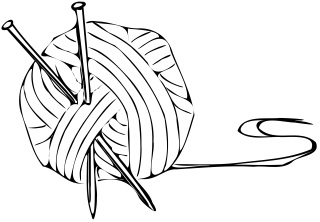
\includegraphics[scale=0.5]{Figures/example}
	\caption[MMCG specimen]{dimensions and geometry of Mixed Mode Crack Growth specimen}
	\label{fig:Fig5}
\end{figure}
MMCG sample is a compromise between DCB and CTS samples to obtain different mixing rates and a stable crack propagation. The choice was made regarding to the good stability of the crack propagation. The Geometry, visible on \ref{fig:Fig5} was already tested in \cite{Reference7} works. The chosen MMCG specimens are Radial and Tangential surface specimens looking to the orthotropic directions of wood. The Tangential direction corresponds to the thickness involving an important swelling of this thickness depending on the Moisture Content.



%\\\\\\\\\\\\\\\\\\\\\\\\\\\\\\\\\\\\\\\\\\\\\\\\\\\\\\\\\\

%New chapter

%\\\\\\\\\\\\\\\\\\\\\\\\\\\\\\\\\\\\\\\\\\\\\\\\\\\\\\\\\\

\subsection{Moisture content}\label{Ss:mm}

To determinate the MC in each specimen at a given time, the formula \ref{eq:Moisture content depending on weight} is used.  
\begin{equation}
	H=\frac{_{M_{S}-M_{0}}}{M_{0}}100
	\label{eq:Moisture content depending on weight}
\end{equation} 

The scale used to weight the specimen was the GR-200 which is a Semi-Micro Analytical Balances. The maximum weight of the denser wood, the Padouck, is around 70.5\si{gram} and the minimum weight of Okoume specimens is 36\si{gram}
After drying the specimens during 24h at 103\textcelsius, in order to obtain the $M_{0}$ parameter, the current MC in the specimens was determinated. 
The average moisture content is around 9.20\% for Okoume specimens and 6.10\% for Padouck specimens at room conditions.
Then, to test specimens at 3 different MC, a system was designed in order to increase the MC.
After 80.62h under water, almost all the specimens were saturated, except some Padouck specimen, denser so with less space for water progression.

During the increase/decrease process, it appears that both species, Okoume and Padouck, earn a constant MC. The difference is the value of this constant increasing. Okoume specimens earn approximately 5\% MC each day, while Padouck ones earn around 2\% MC.


But wood is a living material with a really particular behavior. So the tests were done at 7\% for Okoume and 5\% for Padouck in Room temperature, but for tests at 20\% it was at 19\% for Okoume and 15\% for Padouck, concerning tests at 30\% it was finally at 26\% for Okoume and 21\% for Padouck.

%\\\\\\\\\\\\\\\\\\\\\\\\\\\\\\\\\\\\\\\\\\\\\\\\\\\\\\\\\\

%New chapter

%\\\\\\\\\\\\\\\\\\\\\\\\\\\\\\\\\\\\\\\\\\\\\\\\\\\\\\\\\\

\subsection{Opening mode fracture loading}\label{Ss:modeIfrac}


%\\\\\\\\\\\\\\\\\\\\\\\\\\\\\\\\\\\\\\\\\\\\\\\\\\\\\\\\\\

%New chapter

%\\\\\\\\\\\\\\\\\\\\\\\\\\\\\\\\\\\\\\\\\\\\\\\\\\\\\\\\\\

\subsubsection{Compliance method}\label{Ss:complmet}

To determine the Energy release rate and compare specimens regarding the specie and the MC, compliance method was chosen. 
The formula used to calculate this energy release rate is written on \ref{eq:Energy release rate equation}:
\begin{equation}
	G_{c}= \frac{F_{c}^2}{2b} (\frac{\Delta C}{\Delta a})_{d} 	
	\label{eq:Energy release rate equation}
\end{equation}  
With : 
$G_c$ the value of energy release rate (in \si{\joule\per\square\meter})
$F_c$ the critical force which involves the crack (in \si{\newton})
b the thickness of the specimen (in \si{\milli\meter})
$\Delta C$ the compliance evolution (in $Pa^-1$)
$\Delta a$ the crack length evolution (in \si{\milli\meter})
In this work, C is determined in forced displacement, by the division of U, the imposed displacement, by F, the applied force. It must be noted that this forced displacement was 0,015\si{\milli\meter\per\second} according to some articles, \cite{Reference7} or \cite{reference15} advising 2\si{\milli\meter\per\minute} until 5\si{\milli\meter\per\minute} displacement.
The specimens are Radial/Longitudinal surface so the Tangential dimension represent their thickness. It involves a dimension evolution of "b" parameter. So for each test at a different MC, the b parameter must be measured, in order to have a precise value of G. Compliance method is often used in mode I analysis. It was the way of study for works as \cite{Reference7}, \cite{Ang2017}...

%\\\\\\\\\\\\\\\\\\\\\\\\\\\\\\\\\\\\\\\\\\\\\\\\\\\\\\\\\\

%New chapter

%\\\\\\\\\\\\\\\\\\\\\\\\\\\\\\\\\\\\\\\\\\\\\\\\\\\\\\\\\\

\subsubsection{Fracture tests}\label{Ss:fractests}

%\\\\\\\\\\\\\\\\\\\\\\\\\\\\\\\\\\\\\\\\\\\\\\\\\\\\\\\\\\

%New chapter

%\\\\\\\\\\\\\\\\\\\\\\\\\\\\\\\\\\\\\\\\\\\\\\\\\\\\\\\\\\

\subsection{Digital image correlation}\label{Ss:dic}

To study the fracture propagation, image analysis tool was used.
In this work, Digital Image Correlation (DIC) consists in comparing two images of the same object on load, here MMCG specimen, and have a look to the displacement field, in order to find a match between the two images.
DIC method is based on the principles of mechanical continuity (rigid body mechanics). The system consists of using a digital camera and specialized computer software, in this work, MatchID. Camera is used to capture consecutive images of the tested sample surface during the deformation test. Digital images determined by this way, which corresponds to a series of photos, is analyzed by the DIC software. Displacement maps of specimen on the surface is created. Stress fields can be evaluated from strain fields. 

For wood study, it is important to note that elastic orthotropic material model in 2D has five engineering constants as input parameters, to enter in the image analysis system. First, Young modulus in longitudinal direction must be informed, $E_{L}$=$E_{1}$, transverse Young modulus $E_{trans}=E_{R}=E_{T}=E_{2}$ and then, shear modulus $G_{LR}=G_{LT}=G_{12}$. Therefore, Poisson coefficient $\nu$ has to be put into the software. Focusing on mode I damage, it is described by damage initiation stress $\sigma_{ini}$, but also separation at the failure $\delta_{fl}$, and exponential function shape coefficient $\alpha_{I}$. The following table show the used values for this work.

%\\\\\\\\\\\\\\\\\\\\\\\\\\\\\\\\\\\\\\\\\\\\\\\\\\\\\\\\\\

%New chapter

%\\\\\\\\\\\\\\\\\\\\\\\\\\\\\\\\\\\\\\\\\\\\\\\\\\\\\\\\\\

\subsubsection{Optical set-up and settings}\label{Ss:optical}

An Allied Vision Manta 505B 2/3'' camera coupled to an Opto Engineering TC 23 36 telecentric lens were used for image formation and acquisition. The camera is equipped with Charge-Coupled Device (CCD) sensor with pixel resolution of 2452 (H) $\times$ 2056 (V) (5MP) and sensor size of 2/3''. The monovision camera-lense optical system was fixed on a tripod and its spatial position oriented with regard to the target surface of interest. The telecentric lens has a magnification factor of \num{0.243}$\times$, allowed to image a field of view, in the object space, of 36.2$\times$27.1 \si{\milli\meter\squared}. The front of the lens was positioned at a working distance of 103.5 \si{\milli\meter} with an aperture of $f$/8, yielding a field of depth of 11 \si{\milli\meter}.

A high power adjustable ring light was used to illuminate the region of interest. A monochromatic version corresponding to a green wavelength of \num{525} \si{\nano\meter} was used from which the highest spectral response of the camera sensor will be expected.

All the specimens were painted to obtain a speckle pattern suitable for image correlation. A thin layer of white paint was firstly added using a mate spray, followed by a diffuse distribution of black paint to create a unique local pattern across the region of interest at the crack tip (Figure~\ref{fig:Fig17}).

\begin{figure}[t]
	\centering
	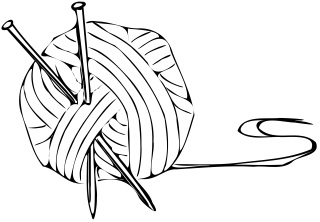
\includegraphics[width=.9\textwidth]{Figures/example}
	\caption{(a) Speckle pattern typically obtained for DIC measurements (2452 $\times$ 2056
		pixels\textsuperscript{2}); (b) Histogram
		of the
		speckle image
		(256
		gray levels, 8 bits camera).}
	\label{fig:Fig17}
\end{figure}

The DIC setting parameters can have a significant influence on the kinematic fields obtained by image correlation (\textit{e.g.} subset size, subset step, \ldots) and numerical differentiation (\textit{e.g.} strain windows size) algorithms \cite{Pereira2018566}. These settings represent fundamental parameters since they will define the spatial resolution and accuracy associated to the DIC measurements, both in displacement and strain fields.  Therefore, a parametric study was carried out to justify the DIC setting for the current
application, in a balance between resolution and spatial resolution. This study was carried ot in the Parametric Module of MatchID 2D software.
\begin{table}[]
	\centering
	\begin{tabular}{c c}
		\hline
		Correlation   Coefficient: & ZNSSD \\ 
		Interpolation order: & Bicubic Splines \\ 
		Transformation order: & Affine \\
		Subset size: & 21 \\
		Step size: & 5 \\
		Maximum rigid body estimation: & 100 \\ 
		Strain Estimation(\%): & 5 \\ 
		Precision: & 0.001 \\ 
		Maximum iterations: & 20 \\ 
		Noise handling: & Gaussian \\ 
		Kernel Size: & 5 \\ 
		History: & Spatial \\ 
		Strainwindow size: & 7 \\ 
		Tolerance on number of points: & 0 \\ 
		Strain interpolation: & Q4 \\ 
		Strain Convention: & Green-Lagrange \\ \hline
	\end{tabular}
	\caption{MatchID parameters used}
	\label{tab:MatchID_param}
\end{table}
\ref{tab:MatchID_param} defines the range of values defined in this performance analysis which includes the subset size ($f_s$), subset step, affine and quadratic displacement shape functions, the strain windows size and the order of the polynomial fitting function. The pre-selected range of values are deemed to be representative of the range of acceptable DIC setting parameters. For instance, The lower pixel boundary is constrained by aliasing effects, which is a function of the speckle size on the imaged pattern. The subset size defines the target matching pattern used in the correlation algorithm. A rule of thumb will be three contrasted speckles per subset. The average speckle size was determined as 4.5 pixels. Therefore, the minimum subset step was set to 15 pixels. The upper pixel limit can be problem-dependent, taking into account the deformation gradients expected within the region of interest, in a balance between spatial resolution and resolution. As a guideline, larger subsets improves the resolution but decreases spatial resolution. Parameters such as the subset step ($f_p$) (distance between centroids of adjacent subsets, units: pixels) and the strain window $\varepsilon_w$ (number of subsets central points used to define a mesh of data points over which a piecewise polynomial fitting will be applied, using least-square regression, for strain reconstruction) will define a strain spatial resolution ($\Delta \varepsilon$) and virtual strain gauge (VSG), respectively, according to the following relationships \cite{Lava2013576,Pereira2018566}: $\Delta \varepsilon = (\varepsilon_w-1)f_p + f_s$ and $\mbox{VSG} = (\varepsilon_w-1)f_p + 1$ (unit: pixel). For convenience, these parameters can be converted to physical units in the object space (\textit{e.g.} mm), by simple multiplication by the conversion factor of the optical imaging system. All these external DIC parameters, therefore, must be carefully selected in the current study.


Here, all the matrix, composed of the subsets from the Zone of Interest are changed by the different steps shown overhead. All the subsets are considered four by four and the displacement from one compared to it neighbor are computed. Then average and maximum values are obtained for each subset of the ZOI and put into a matrix (named K overhead). By using the $a_{0}$ data and looking to an alpha parameter, the programm compute the best shape of a(t). Alpha parameter allow to avoid the image noise but is close enough to give precise a(t) values.
This method was the one used by \cite{Reference14} on MatLab, and have already proved obtention of good results.

%\\\\\\\\\\\\\\\\\\\\\\\\\\\\\\\\\\\\\\\\\\\\\\\\\\\\\\\\\\

%New chapter

%\\\\\\\\\\\\\\\\\\\\\\\\\\\\\\\\\\\\\\\\\\\\\\\\\\\\\\\\\\


As shown in the code, the dimensions of the matrix take in account the number of stages, so the number of images. Indeed, the interest of the CTOD is to be followed at each stage. 

Then, a loop is created, allowing to put information into others vectors

Another one is also created to compared to mode II values. In the current case, the mode II can be approximate around zero, because it is a mode I test. Then all the values are obtained, for each COD pair until $ud_lim$ which is in this case equal to 10. By looking to this different curves, the chosen COD pair is chosen and a curve is plot looking to the values for this parameter chosen by the user. 

\begin{figure}[h]
	\centering
	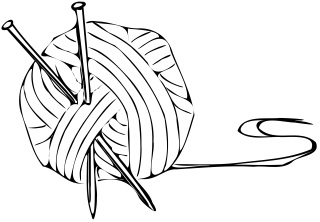
\includegraphics[scale=0.7]{Figures/example}
	\caption[Subset choice and pair of subset around]{Pair of subset around the $a_{0}$ subset chosen}
	\label{fig:subest_chosen}
\end{figure}

Finally, the way to obtain CTOD, need also a well $a_{0}$ choice. Indeed, the chosen subset as presented on \ref{fig:subest_chosen}, will be determinant. Considering the image as a matrix composed of subset, the chosen subset as a position given by his m row and n column. To determinate the opening, it is necessary to have a look on the subsets in the same n column but at a different line. Indeed, the chosen subset will be the first one affected by the crack, that means, that information on the subset will not have importance anymore. While, looking to subset up and down allow to follow the displacement of the crack tip and measure it. The fact is to determine which pair of subsets is the best. The ones at the row n-1 and n+1, but maybe these ones will be on the crack at a given stage, and will lose all the necessary information. That is why, an important choice must be done. Here, COD pair was fixed equal to two. So the subset displacement analysed is the one of the pair of subset 2 on \ref{fig:subest_chosen}. Finally, by looking to these displacements, it is possible to obtain the value of the crack opening at each stages.

%\\\\\\\\\\\\\\\\\\\\\\\\\\\\\\\\\\\\\\\\\\\\\\\\\\\\\\\\\\

%New chapter

%\\\\\\\\\\\\\\\\\\\\\\\\\\\\\\\\\\\\\\\\\\\\\\\\\\\\\\\\\\

\section{Results}\label{S:res}
\subsection{Maximum Load}\label{S:pdcurves}

The first results, obtained with the servohydraulic press were, as presented in \ref{fig:Res_Pmax}, the necessary loads to involve a propagation of the crack in all the ZOI and sometimes until the entire destruction of the specimen.

\begin{figure}[th]
	\centering
	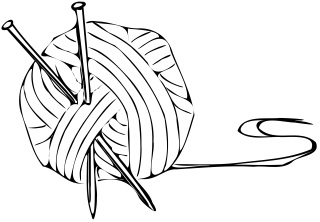
\includegraphics[width=\textwidth]{Figures/example}
	\caption[Maximal load reach for each specimen]{Maximal load reach for each specimen compared to the Moisture Content of the specimens}
	\label{fig:Res_Pmax}
\end{figure}

As expected, Padouck specimens need a higher load to involve the final crack. It was obvious, that the denser material is more difficult to destroy than the lower one.

%\\\\\\\\\\\\\\\\\\\\\\\\\\\\\\\\\\\\\\\\\\\\\\\\\\\\\\\\\\

%New chapter

%\\\\\\\\\\\\\\\\\\\\\\\\\\\\\\\\\\\\\\\\\\\\\\\\\\\\\\\\\\


\section{Discussion}\label{S:dis}

This work is really interesting compared to previous ones. In every works the MC increase phenomenon decrease the Resistance of the material. The G and the $\sigma$ were obtained on European species and this trend was confirmed. But since the beginning of tests on Tropical species, others behavior are found. \cite{Reference7} has proved by his work, that the results, regarding to the mode and the load angle applied, for Iroko, Okoume and Padouck, are similar to European ones. But no proof were already done concerning the behavior of this species to MC effect. This species from Gabon are submitted to higher temperature and relative humidity around 80\%. And looking to work as \cite{Kif1998} and \cite{Ang2017}, the density of Scots Pine and Douglas, can be compared to Okoume specimens, and then the results from these specimens can be discussed. It appears that the early wood more saturated in water than the lately one involves a decrease of the $\sigma$. A similar trend is shown on Douglas Fir regarding two MC values, 9\% and 18\%. The fact is that the Okoume species do not have this trend and is stable.



%\\\\\\\\\\\\\\\\\\\\\\\\\\\\\\\\\\\\\\\\\\\\\\\\\\\\\\\\\\

%New chapter

%\\\\\\\\\\\\\\\\\\\\\\\\\\\\\\\\\\\\\\\\\\\\\\\\\\\\\\\\\\

\section{Conclusions}\label{S:con}

Finally, by analyzing the behavior of Padouk and Okoume species submitted to different moisture content, this study has shown how this climatic effect can affect wood fracture mechanics.
\newline
The tests done at different moisture contents for several MMCG geometry specimens, coupled to the use of DIC with MatchID software and python processing were determinant to obtained results.
The results shown and the interpretation can be discussed, but according to this work, Padouck seems to have better characteristics at 15\% moisture content, before a decrease of the energy release rate with the 20\% moisture content treeshold overrun. 
\newline
By changing one parameter as the moisture content or the species, it will be possible to reuse the developed Python code and many determined parameters, in order to find a pattern linking moisture content to fracture mechanics in mode 1.

%\begin{table}[h]
%\caption{An example of a table.}
%\begin{tabular*}{\hsize}{@{\extracolsep{\fill}}lll@{}}
%\toprule
%An example of a column heading & Column A ({\it{t}}) & Column B ({\it{t}})\\
%\colrule
%And an entry &   1 &  2\\
%And another entry  & 3 &  4\\
%And another entry &  5 &  6\\
%\botrule
%\end{tabular*}
%\end{table}

%\enlargethispage{12pt}

%Reference generation by using bibliography style commands for LaTeX template only.
%
%The author may use ``elsarticle-harv.bst'' as per the style required in document. The sample bib file could be referred.
%If the author may using bibstyle for providing references author must comment the bibliography section in TeX file, Bibtex will generate the reference automatically.
%
%If the author may not able to view the references in output same could be done by copying the bibliography section from ``filename.bbl'' file and paste in TeX file.


\subsection{General guidelines for the preparation of your text}
Avoid hyphenation at the end of a line. Symbols denoting vectors and matrices should be indicated in bold type. Scalar variable names should normally be expressed using italics. Weights and measures should be expressed in SI units. All non-standard abbreviations or symbols must be defined when first mentioned, or a glossary provided.

%\begin{figure}[t]\vspace*{4pt}
%%\centerline{\includegraphics{fx1}\hspace*{5mm}\includegraphics{fx1}}
%\centerline{\includegraphics{gr1}}
%\caption{(a) first picture; (b) second picture.}
%\end{figure}

%\begin{equation}
%\begin{array}{lcl}
%\displaystyle X_r &=& \displaystyle\dot{Q}^{''}_{rad}\left/\left(\dot{Q}^{''}_{rad} + \dot{Q}^{''}_{conv}\right)\right.\\[6pt]
%\displaystyle \rho &=& \displaystyle\frac{\vec{E}}{J_c(T={\rm const.})\cdot\left(P\cdot\left(\displaystyle\frac{\vec{E}}{E_c}\right)^m+(1-P)\right)}
%\end{array}
%\end{equation}

\section*{Acknowledgements}

This research was funded by the project UIDB/00667/2020 (UNIDEMI) supported
by Fundação para a Ciência e a Tecnologia (FCT-MCTES), the Portuguese
national funding agency for science, research and technology.

%% The Appendices part is started with the command \appendix;
%% appendix sections are then done as normal sections
%% \appendix

%% \section{}
%% \label{}

%\appendix
%\section{An example appendix}
%Authors including an appendix section should do so before References section. Multiple appendices should all have headings in the style used above. They will automatically be ordered A, B, C etc.
%
%\subsection{Example of a sub-heading within an appendix}
%There is also the option to include a subheading within the Appendix if you wish.

%% References
%%
%% Following citation commands can be used in the body text:
%% Usage of \cite is as follows:
%%   \cite{key}         ==>>  [#]
%%   \cite[chap. 2]{key} ==>> [#, chap. 2]
%%

%The citation must be used in following style: \cite{article-minimal} \cite{article-full} \cite{article-crossref} \cite{whole-journal}.
%% References with BibTeX database:

\bibliography{biblio}
\bibliographystyle{elsarticle-harv}

%% Authors are advised to use a BibTeX database file for their reference list.
%% The provided style file elsarticle-num.bst formats references in the required Procedia style

%%% For references without a BibTeX database:
%
% \begin{thebibliography}{}
%
%%% \bibitem must have the following form:
%%%   \bibitem{key}...
%%%
%
%\bibitem[Clark et al.(1962)]{clark}Clark, T., Woodley, R.,
%De Halas, D., 1962. Gas-Graphite Systems, in ``{\it
%Nuclear
%Graphite}''.
%In: Nightingale, R. (Ed.). Academic Press, New York, pp.
%387.
%
%\bibitem[Deal and Grove(2009) ]{Deal}Deal, B., Grove, A.,
%1965. General Relationship for the Thermal Oxidation of
%Silicon. Journal of Applied Physics 36, 37--70.
%
%\bibitem[Deep(2009)]{Deep}Deep-Burn Project: Annual Report
%for 2009, Idaho National Laboratory, Sept. 2009.
%
%\bibitem[Fachinger(2004)]{Fachinger2004}Fachinger, J., den
%Exter, M., Grambow, B., Holgerson, S., Landesmann, C.,
%Titov, M., Podruhzina, T., 2004. ``Behavior of spent HTR
%fuel elements in aquatic phases of repository host rock
%formations,'' 2nd International Topical Meeting on High
%Temperature Reactor Technology. Beijing, China, paper
%\#B08.
%
%\bibitem[Fachinger(2006)]{Fachinger2006}Fachinger, J.,
%2006. Behavior of HTR Fuel Elements in Aquatic Phases of
%Repository Host Rock Formations. Nuclear Engineering \&
%Design 236,     54.
%
%
% \end{thebibliography}
%
%\clearpage

%%%% This page is for instructions only, once the article is finalize please omit the below text before creating the final PDF
%\normalMode
%
%\section*{Instructions to Authors for LaTeX template:}
%
%\section{ZIP mode for LaTeX template:}
%
%The zip package is created as per the guide lines present on the URL http://www.elsevier.com/author-schemas/ preparing-crc-journal-articles-with-latex for creating the LaTeX zip file of Procedia LaTeX template.  The zip generally contains the following files:
%\begin{Itemize}[]\leftskip-17.7pt\labelsep3.3pt
%\item ecrc.sty
%\item  elsarticle.cls
%\item elsdoc.pdf
%\item .bst file
%\item Manuscript templates for use with these bibliographic styles
%\item  Generic and journal specific logos, etc.
%\end{Itemize}
%
%The LaTeX package is the main LaTeX template. All LaTeX support files are required for LaTeX pdf generation from the LaTeX template package.
%
%{\bf Reference style .bst file used for collaboration support:} In the LaTeX template packages of all Procedia titles a new ``.bst'' file is used which supports collaborations downloaded from the path http://www.elsevier.com/author-schemas/the-elsarticle-latex-document-class

\end{document}

%%
%% End of file `prostr-template.tex'.
